% Created 2016-01-08 Fri 16:42
\documentclass[presentation]{beamer}
\usepackage[utf8]{inputenc}
\usepackage[T1]{fontenc}
\usepackage{fixltx2e}
\usepackage{graphicx}
\usepackage{grffile}
\usepackage{longtable}
\usepackage{wrapfig}
\usepackage{rotating}
\usepackage[normalem]{ulem}
\usepackage{amsmath}
\usepackage{textcomp}
\usepackage{amssymb}
\usepackage{capt-of}
\usepackage{hyperref}
\usepackage{minted}
\usepackage{tikz}
\usepgflibrary{shapes.geometric}
\usetikzlibrary{calc}
\usetikzlibrary{positioning}
\beamertemplatenavigationsymbolsempty
\makeatletter
\setbeamertemplate{footline}
{
\leavevmode%
\hbox{%
\begin{beamercolorbox}[wd=\paperwidth,ht=2.25ex,dp=1ex,right]{date in head/foot}%
\hfil\insertframenumber\hspace{2em}
\end{beamercolorbox}}%
\vskip0pt%
}
\makeatother
\usetheme{default}
\author{Lawrence Mitchell, Mark Filipiak\thanks{lawrence.mitchell@ed.ac.uk, mjf@epcc.ed.ac.uk}}
\date{Tuesday 18th March 2013}
\title{Partitioning and numbering meshes for efficient MPI-parallel execution in PyOP2}
\hypersetup{
 pdfauthor={Lawrence Mitchell, Mark Filipiak},
 pdftitle={Partitioning and numbering meshes for efficient MPI-parallel execution in PyOP2},
 pdfkeywords={},
 pdfsubject={},
 pdfcreator={Emacs 24.5.1 (Org mode 8.3.2)}, 
 pdflang={English}}
\begin{document}

\maketitle
\begin{frame}{Outline}
\tableofcontents
\end{frame}

\section{Numbering to be cache friendly}
\label{sec:orgheadline10}

\begin{frame}[label={sec:orgheadline1}]{Modern hardware}
\begin{itemize}
\item Latency to RAM is 100s of clock cycles
\item Multiple caches to hide this latency
\begin{itemize}
\item memory from RAM arrives in cache lines (64 bytes, 128 bytes on
Xeon Phi)
\item hardware prefetching attempts to predict next memory access
\end{itemize}
\end{itemize}
\end{frame}

\begin{frame}[label={sec:orgheadline2}]{Exploiting hardware caches in FE assembly}
\begin{itemize}
\item Direct loops over mesh entities are cache-friendly
\item indirect loops may not be
\begin{itemize}
\item can we arrange them to be cache friendly?
\end{itemize}
\end{itemize}
\end{frame}

\begin{frame}[label={sec:orgheadline3}]{A mesh}
\begin{center}
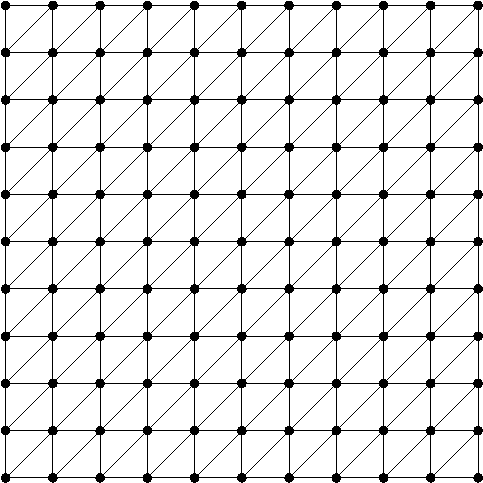
\includegraphics[width=7cm]{03-18-FEniCS-mesh-numbering.figures/mesh}
\end{center}
\end{frame}

\begin{frame}[label={sec:orgheadline4}]{Cache friendly visit order (default numbering)}
\begin{center}
\only<1>{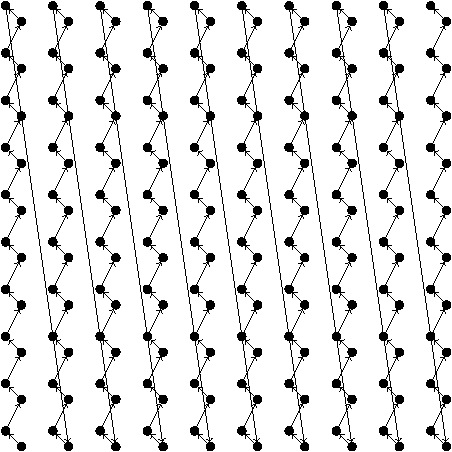
\includegraphics[width=6cm]{03-18-FEniCS-mesh-numbering.figures/bad-elements}}
\only<2>{\vspace{2em}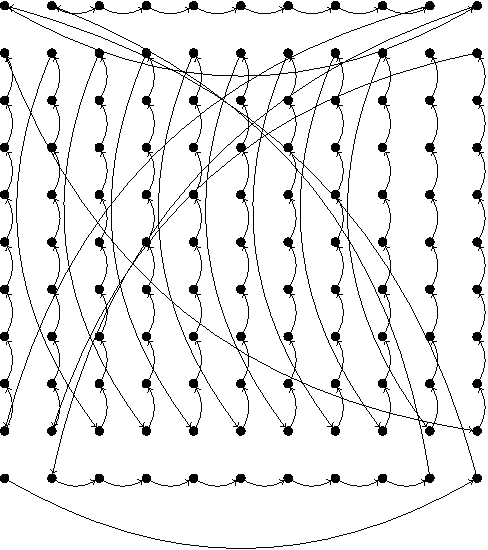
\includegraphics[width=6cm]{03-18-FEniCS-mesh-numbering.figures/bad-nodes}}
\only<3>{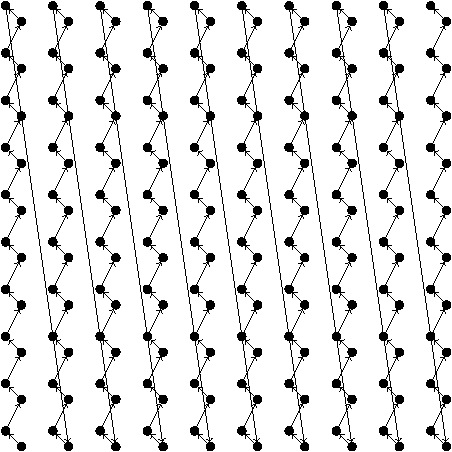
\includegraphics[width=4.5cm]{03-18-FEniCS-mesh-numbering.figures/bad-elements}\hspace{2em}
         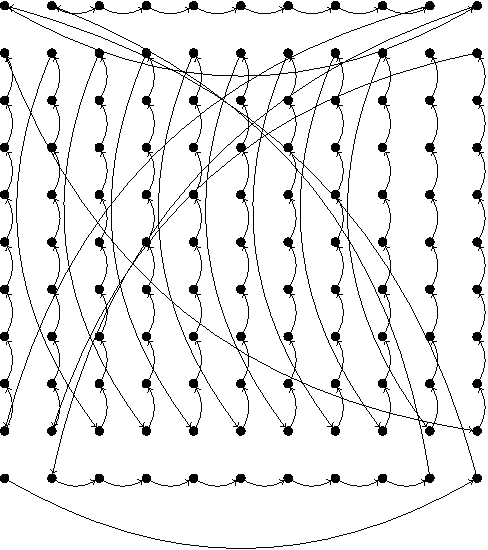
\includegraphics[width=4.5cm]{03-18-FEniCS-mesh-numbering.figures/bad-nodes}}
\end{center}
\end{frame}

\begin{frame}[label={sec:orgheadline5}]{Mesh entity numbering is critical}
\begin{itemize}
\item arrange for ``connected'' vertices to have a good numbering (close to
each other)
\item given this good numbering
\begin{itemize}
\item derive numberings for other entities
\end{itemize}
\end{itemize}
\end{frame}

\begin{frame}[label={sec:orgheadline6}]{Numbering dofs}
\begin{itemize}
\item Cover mesh with space-filling curve
\begin{itemize}
\item vertices that are close to each other get close numbers
\end{itemize}
\end{itemize}

\begin{center}
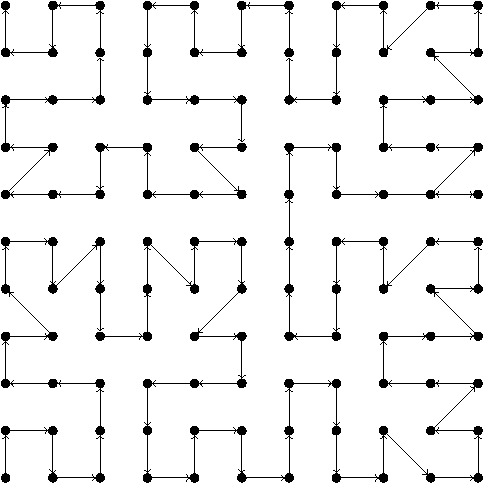
\includegraphics[width=7cm]{03-18-FEniCS-mesh-numbering.figures/good-nodes}
\end{center}
\end{frame}

\begin{frame}[label={sec:orgheadline7}]{Other entities}
\begin{itemize}
\item construct additional entities with some numbering
\item sort them and renumber lexicographically keyed on sorted list of
vertices they touch
\item do this every time the mesh topology changes
\begin{itemize}
\item (doesn't work yet)
\end{itemize}
\end{itemize}
\begin{center}
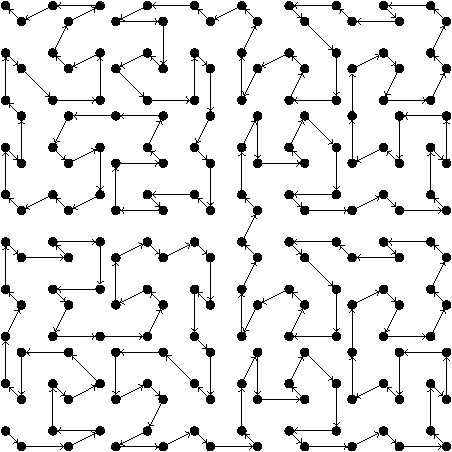
\includegraphics[width=7cm]{03-18-FEniCS-mesh-numbering.figures/good-elements}
\end{center}
\end{frame}

\begin{frame}[label={sec:orgheadline8}]{Comparing}
\begin{center}
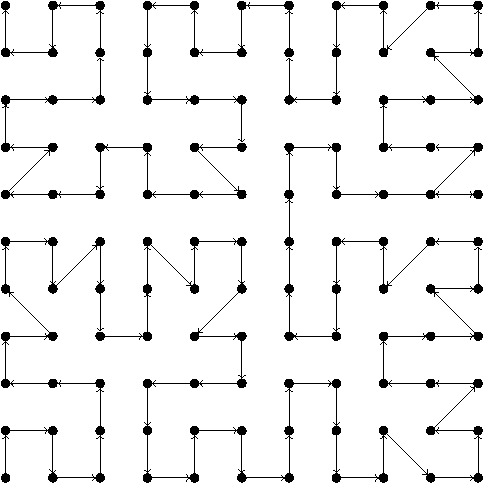
\includegraphics[width=3.8cm]{03-18-FEniCS-mesh-numbering.figures/good-nodes}\hspace{2em}
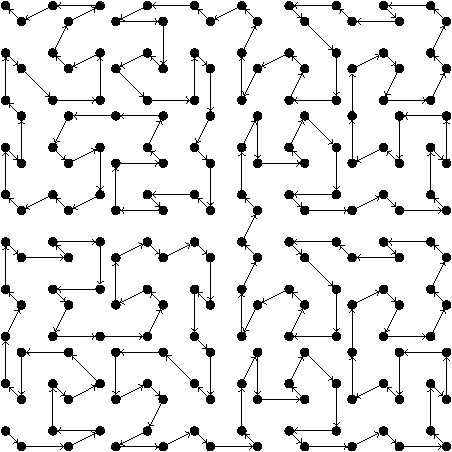
\includegraphics[width=3.8cm]{03-18-FEniCS-mesh-numbering.figures/good-elements}\vspace{1em}
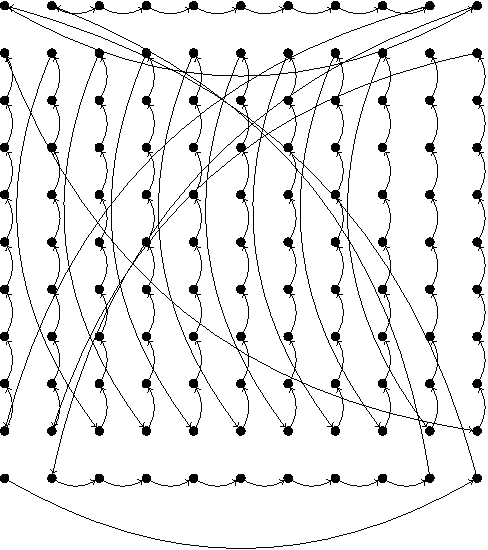
\includegraphics[width=3.8cm]{03-18-FEniCS-mesh-numbering.figures/bad-nodes}\hspace{2em}
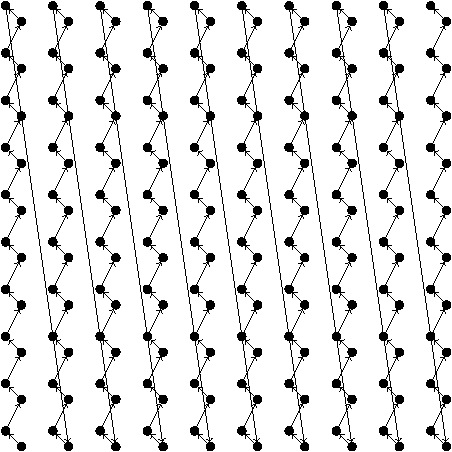
\includegraphics[width=3.8cm]{03-18-FEniCS-mesh-numbering.figures/bad-elements}
\end{center}
\end{frame}

\begin{frame}[label={sec:orgheadline9}]{Does it work?}
\begin{itemize}
\item In Fluidity
\begin{itemize}
\item P1 problems get around 15\% speedup
\end{itemize}
\item In PyOP2
\begin{itemize}
\item GPU/OpenMP backends get 2x-3x speedup (over badly numbered case)
\item Fluidity kernels provoke cache misses in other ways
\end{itemize}
\end{itemize}
\end{frame}

\section{Numbering for parallel execution}
\label{sec:orgheadline18}
\begin{frame}[label={sec:orgheadline11}]{Iteration in parallel}
\begin{itemize}
\item Mesh distributed between MPI processes
\item communicate halo data
\item would like to overlap computation and communication
\end{itemize}
\end{frame}

\begin{frame}[label={sec:orgheadline12}]{Picture}
\begin{center}
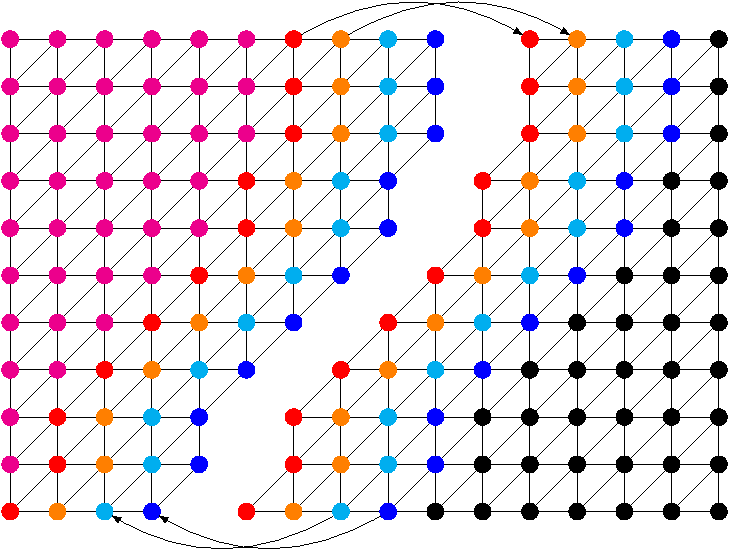
\includegraphics[width=\textwidth]{03-18-FEniCS-mesh-numbering.figures/mpi-mesh}
\end{center}
\end{frame}
\begin{frame}[fragile,label={sec:orgheadline13}]{Comp/comms overlap}
 \begin{itemize}
\item entities that need halos can't be assembled until data has arrived
\item can assemble the other entities already
\end{itemize}
\begin{minted}[frame=none,xleftmargin=1em,xrightmargin=1em,fontsize=\scriptsize,mathescape]{python}
start_halo_exchanges()
for e in entities:
    if can_assemble(e):
        assemble(e)
finish_halo_exchanges()
for e in entities:
    if still_needs_assembly(e):
        assemble(e)
\end{minted}
\end{frame}

\begin{frame}[fragile,label={sec:orgheadline14}]{Making this cheap}
 \begin{itemize}
\item separate mesh entities into groups
\end{itemize}
\begin{minted}[frame=none,xleftmargin=1em,xrightmargin=1em,fontsize=\scriptsize,mathescape]{python}
start_halo_exchanges()
for e in core_entities:
    assemble(e)
finish_halo_exchanges()
for e in additional_entities:
    assemble(e)
\end{minted}
\end{frame}

\begin{frame}[label={sec:orgheadline15}]{PyOP2 groups}
\begin{itemize}
\item Core entities
\begin{itemize}
\item can assemble these without halo data
\end{itemize}
\item Owned entities
\begin{itemize}
\item local, but need halo data
\end{itemize}
\item Exec halo
\begin{itemize}
\item off-process, but redundantly executed over (touch local dofs)
\end{itemize}
\item Non-exec halo
\begin{itemize}
\item off-process, needed to compute exec halo
\end{itemize}
\end{itemize}
\end{frame}

\begin{frame}[label={sec:orgheadline16}]{Why like this?}
\begin{itemize}
\item GPU execution
\begin{itemize}
\item launch separate kernels for core and additional entities
\item no branching in kernel to check if entity may be assembled
\end{itemize}
\item Defer halo exchange as much as possible (lazy evaluation)
\end{itemize}
\end{frame}

\begin{frame}[label={sec:orgheadline17}]{How to separate the entities}
\begin{itemize}
\item separate data structures for different parts
\begin{itemize}
\item possible, but hurts direct iterations, and is complicated
\end{itemize}

\item additional ordering constraint
\begin{itemize}
\item core, owned, exec, non-exec
\item implemented in Fluidity/PyOP2
\item each type of mesh entity stored contiguously, obeying this ordering
\end{itemize}
\end{itemize}
\end{frame}

\section{Hybrid shared memory + MPI parallelisation}
\label{sec:orgheadline27}

\begin{frame}[label={sec:orgheadline19}]{Hybrid shared memory + MPI parallelisation}
\begin{itemize}
\item On boundary, assembling off-process entities can contribute to on-process dofs
\item how to deal with this?
\begin{itemize}
\item use linear algebra library that can deal with it
\item e.g. PETSc allows insertion and subsequent communication of
off-process matrix and vector entries
\end{itemize}

\item Not thread safe
\end{itemize}
\end{frame}

\begin{frame}[label={sec:orgheadline20}]{Solution}
\begin{itemize}
\item Do redundant computation
\begin{itemize}
\item this is the default PyOP2 computation model
\end{itemize}
\item Maintain larger halo
\item assemble all entities that touch local dofs
\begin{itemize}
\item turn off PETSc off-process insertion
\end{itemize}
\end{itemize}
\end{frame}

\begin{frame}[label={sec:orgheadline21}]{Picture}
\begin{center}
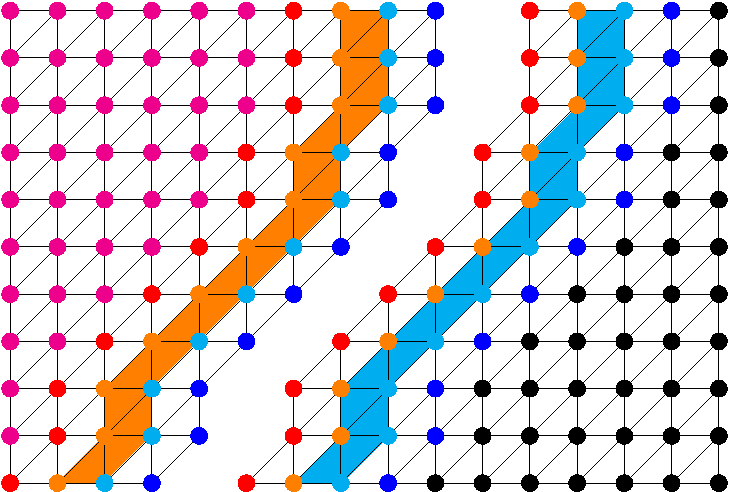
\includegraphics[width=\textwidth]{03-18-FEniCS-mesh-numbering.figures/mpi-mesh-redundant-comp}
\end{center}
\end{frame}

\begin{frame}[label={sec:orgheadline22}]{Multiple gains}
\begin{itemize}
\item You probably did the halo swap anyway
\begin{itemize}
\item this makes form assembly non-communicating
\end{itemize}
\item we've seen significant (40\%) benefit on 1000s of processes
(Fluidity only)
\item thread safety!
\end{itemize}
\end{frame}

\begin{frame}[label={sec:orgheadline23}]{Thread safety}
\begin{itemize}
\item Concurrent insertion into MPI PETSc matrices \emph{is} thread safe if:
\begin{itemize}
\item there's no off-process insertion caching
\item user deals with concurrent writes to rows
\begin{itemize}
\item colour the \emph{local} sparsity pattern
\end{itemize}
\end{itemize}
\end{itemize}
\end{frame}

\begin{frame}[label={sec:orgheadline24}]{Corollary}
\begin{itemize}
\item It is possible to do hybrid MPI/OpenMP assembly with existing
linear algebra libraries
\begin{itemize}
\item implemented (and tested!) in PyOP2
\end{itemize}
\item Ongoing work to add more shared memory parallisation in
kernels in PETSc
\begin{itemize}
\item PETSc team
\item Michael Lange (Imperial)
\end{itemize}
\end{itemize}
\end{frame}

\begin{frame}[label={sec:orgheadline25}]{Conclusions}
\begin{itemize}
\item With a bit a of work, we can make unstructured mesh codes
reasonably cache friendly
\item For good strong scaling, we'd like to overlap computation and
communication as much as possible, but cheaply
\item We think the approaches here work, and are implemented in
Fluidity/PyOP2
\end{itemize}
\end{frame}

\begin{frame}[label={sec:orgheadline26}]{Acknowledgements}
\begin{itemize}
\item Hilbert reordering in Fluidity:
\begin{itemize}
\item Mark Filipiak (EPCC) [a dCSE award from EPSRC/NAG]
\end{itemize}
\item Lexicographic mesh entity numbering and ordering in Fluidity:
\begin{itemize}
\item David Ham (Imperial), and me (prodding him along the way)
\end{itemize}
\item PyOP2 MPI support:
\begin{itemize}
\item me (EPCC) [EU FP7/277481 (APOS-EU)]
\item ideas from Mike Giles and Gihan Mudalige (Oxford)
\end{itemize}
\item MAPDES team:
\begin{itemize}
\item funding (EPSRC grant EP/I00677X/1, EP/I006079/1)
\end{itemize}
\end{itemize}
\end{frame}
\end{document}
